\chapter{Avaliação dos resultados do experimento}
\section{Cenario 1}


\section{Cenario 2}

	\begin{figure}[htb]
	    \centering
		\caption{\label{fig:printSimulacao}Resultado da simulação}
		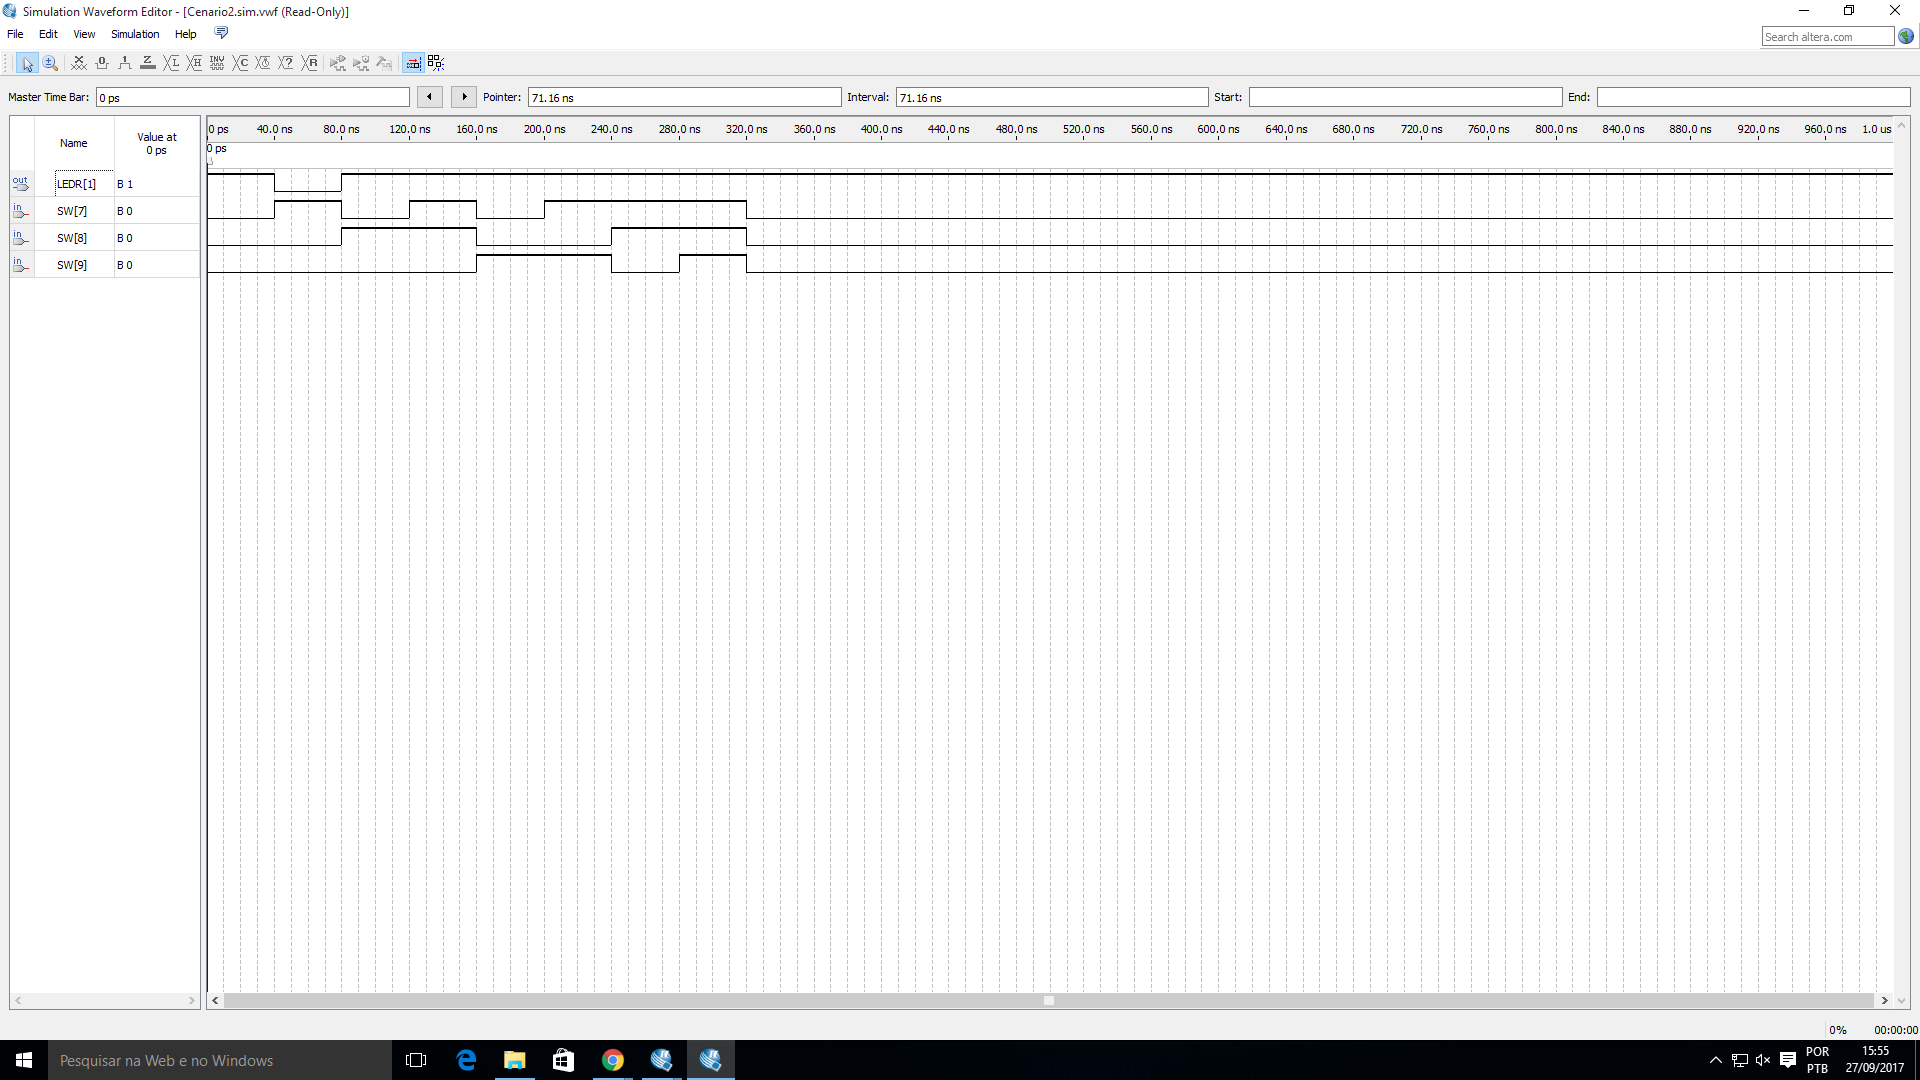
\includegraphics[width=1\textwidth]{img/cenario2/printSimulacao}
	\end{figure}

	\begin{figure}
	    \centering

	    \begin{subfigure}[b]{0.44\textwidth}
	        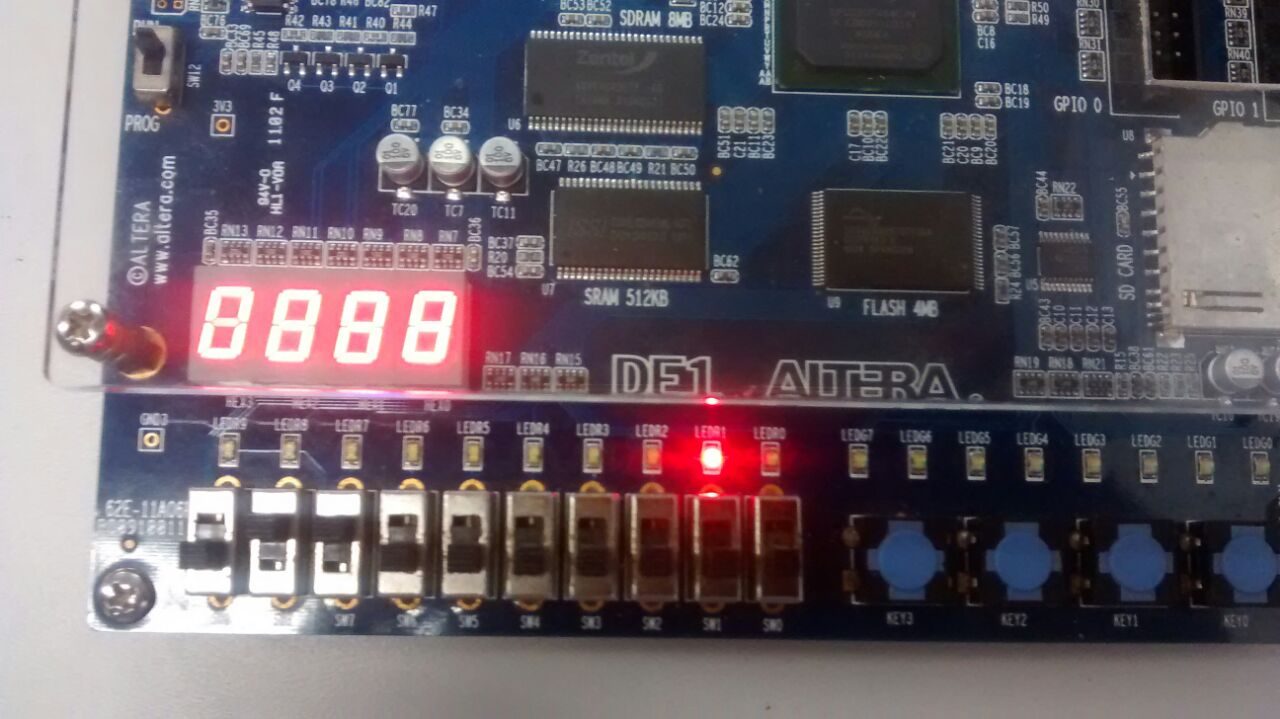
\includegraphics[width=\textwidth]{img/cenario2/circ1}
	        \label{fig:circ1}
			\caption{0 0 0 -> 0}
	    \end{subfigure}
	    ~
	    \begin{subfigure}[b]{0.44\textwidth}
	        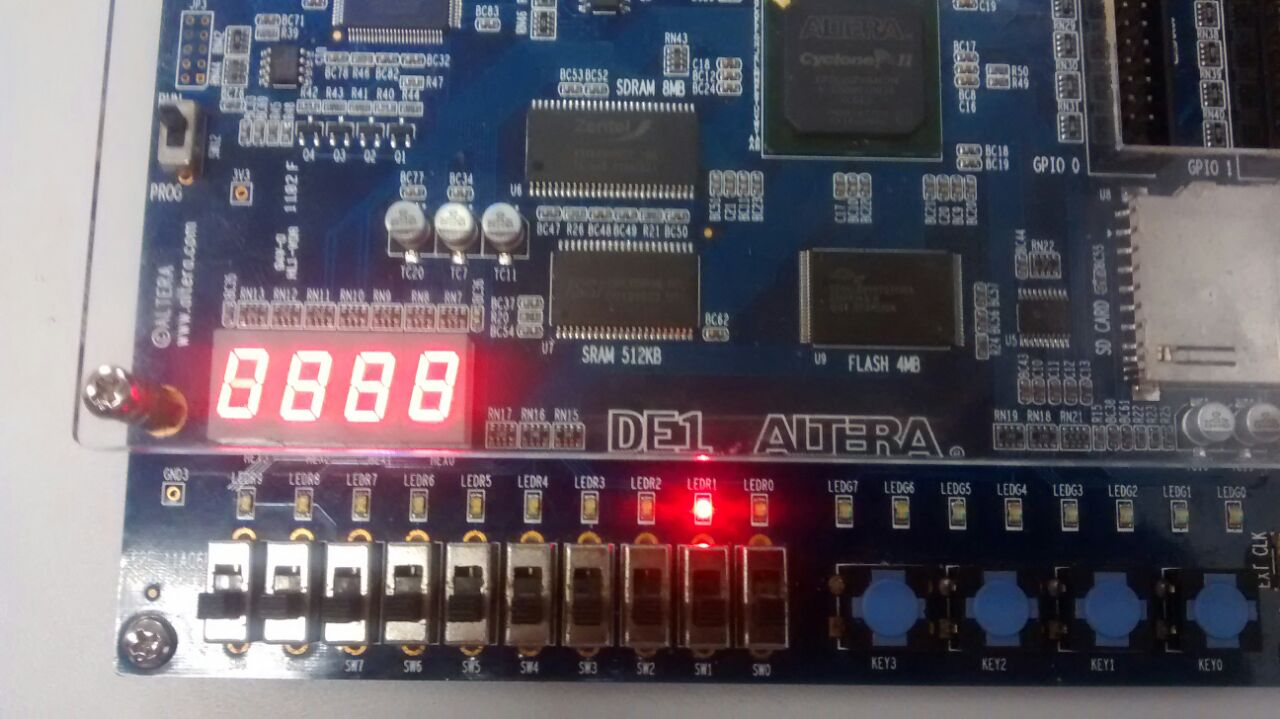
\includegraphics[width=\textwidth]{img/cenario2/circ2}
	        \label{fig:circ2}
			\caption{0 0 1 -> 1}
	    \end{subfigure}


		\begin{subfigure}[b]{0.44\textwidth}
	        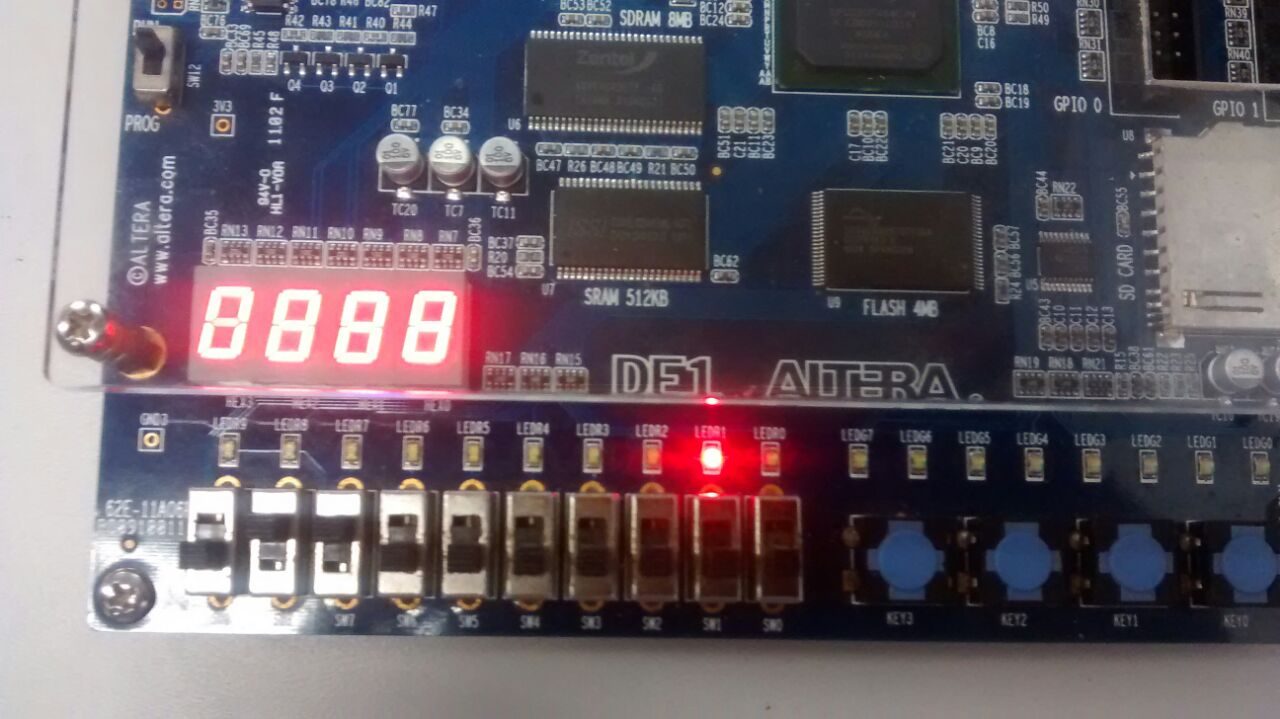
\includegraphics[width=\textwidth]{img/cenario2/circ3}
	        \label{fig:circ3}
			\caption{0 1 0 -> 1}
	    \end{subfigure}
	    ~
	    \begin{subfigure}[b]{0.44\textwidth}
	        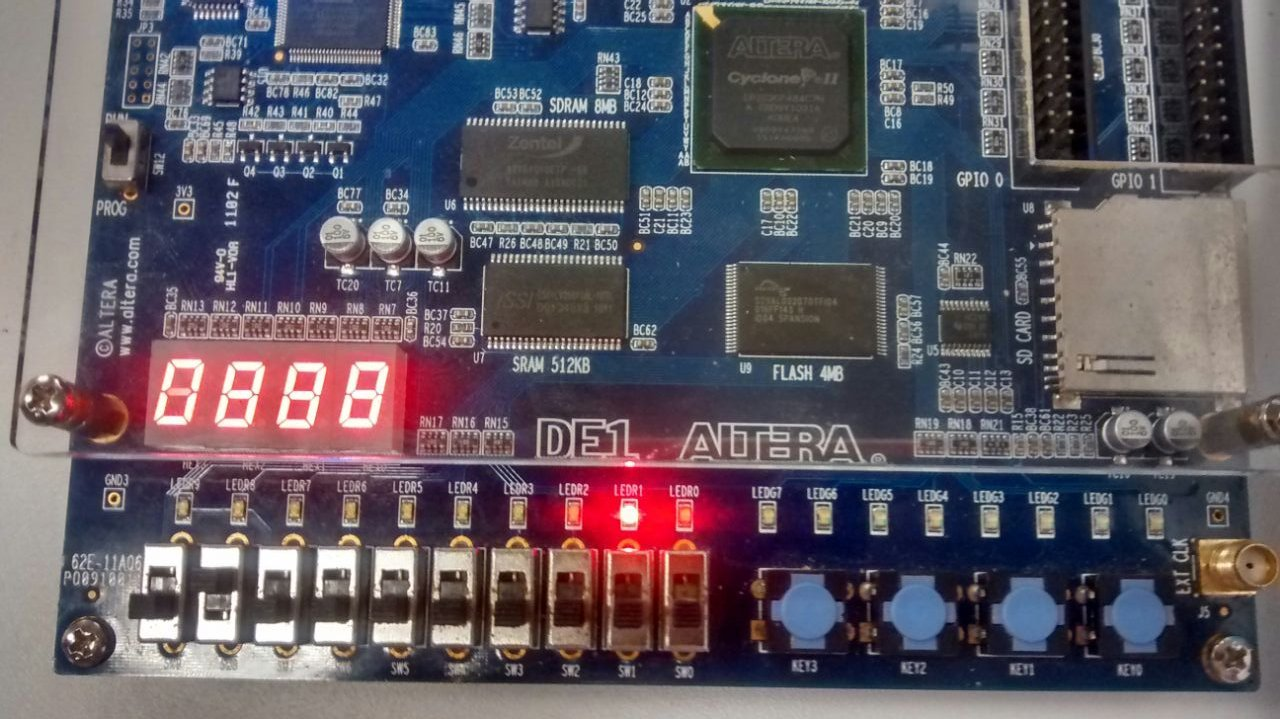
\includegraphics[width=\textwidth]{img/cenario2/circ4}
	        \label{fig:circ4}
			\caption{0 1 1 -> 1}
	    \end{subfigure}


		\begin{subfigure}[b]{0.44\textwidth}
	        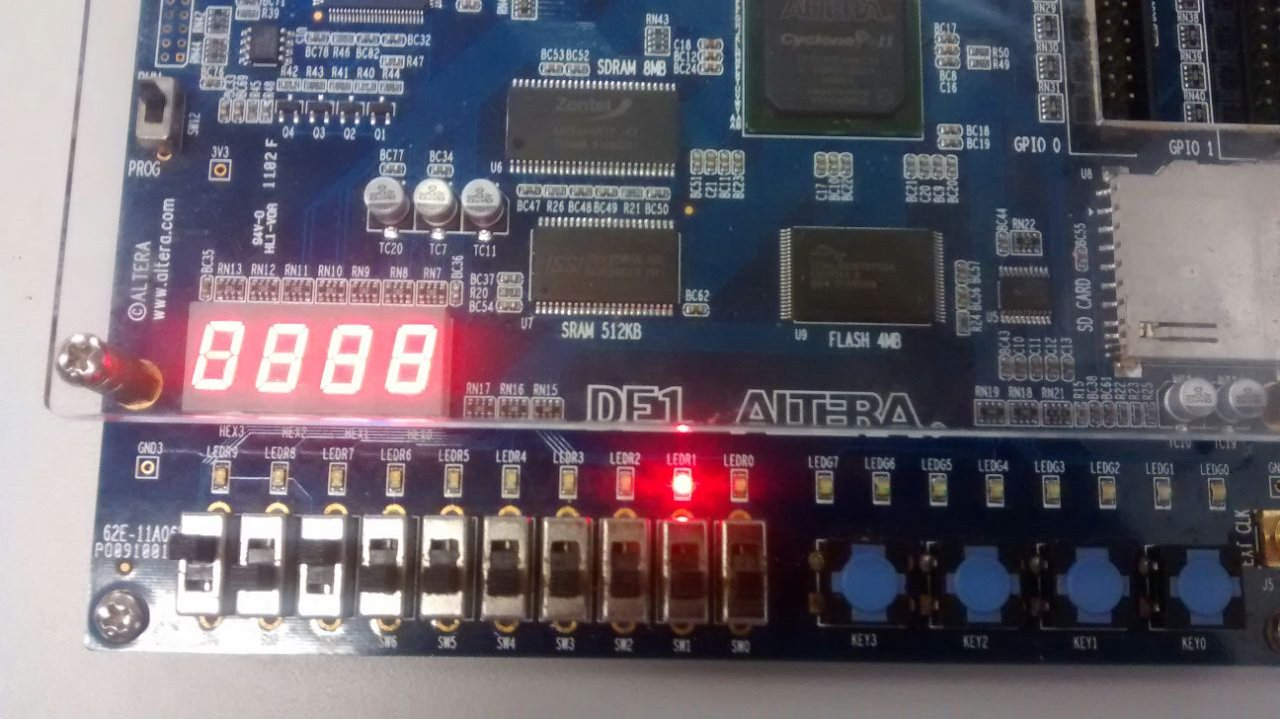
\includegraphics[width=\textwidth]{img/cenario2/circ5}
	        \label{fig:circ5}
			\caption{1 0 0 -> 1}
	    \end{subfigure}
	    ~
	    \begin{subfigure}[b]{0.44\textwidth}
	        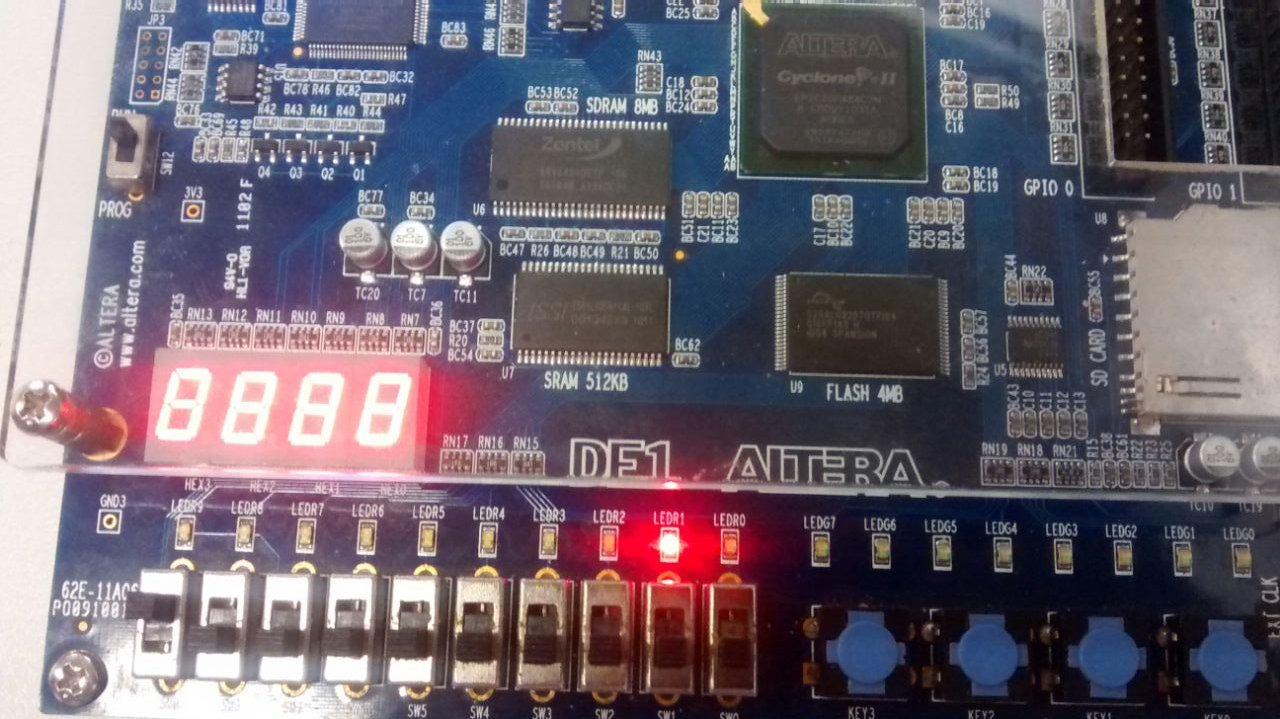
\includegraphics[width=\textwidth]{img/cenario2/circ6}
	        \label{fig:circ6}
			\caption{1 0 1 -> 1}
	    \end{subfigure}

		\begin{subfigure}[b]{0.44\textwidth}
	        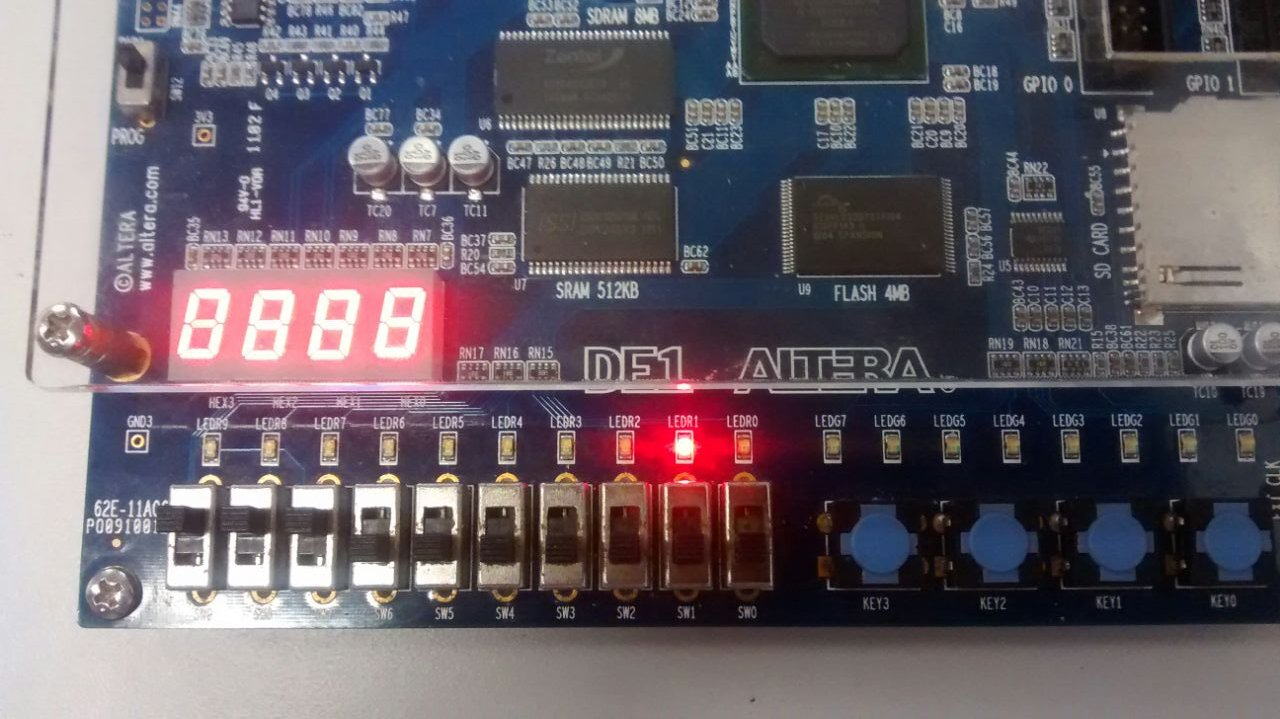
\includegraphics[width=\textwidth]{img/cenario2/circ7}
	        \label{fig:circ7}
			\caption{1 1 0 -> 1}
	    \end{subfigure}
	    ~
	    \begin{subfigure}[b]{0.44\textwidth}
	        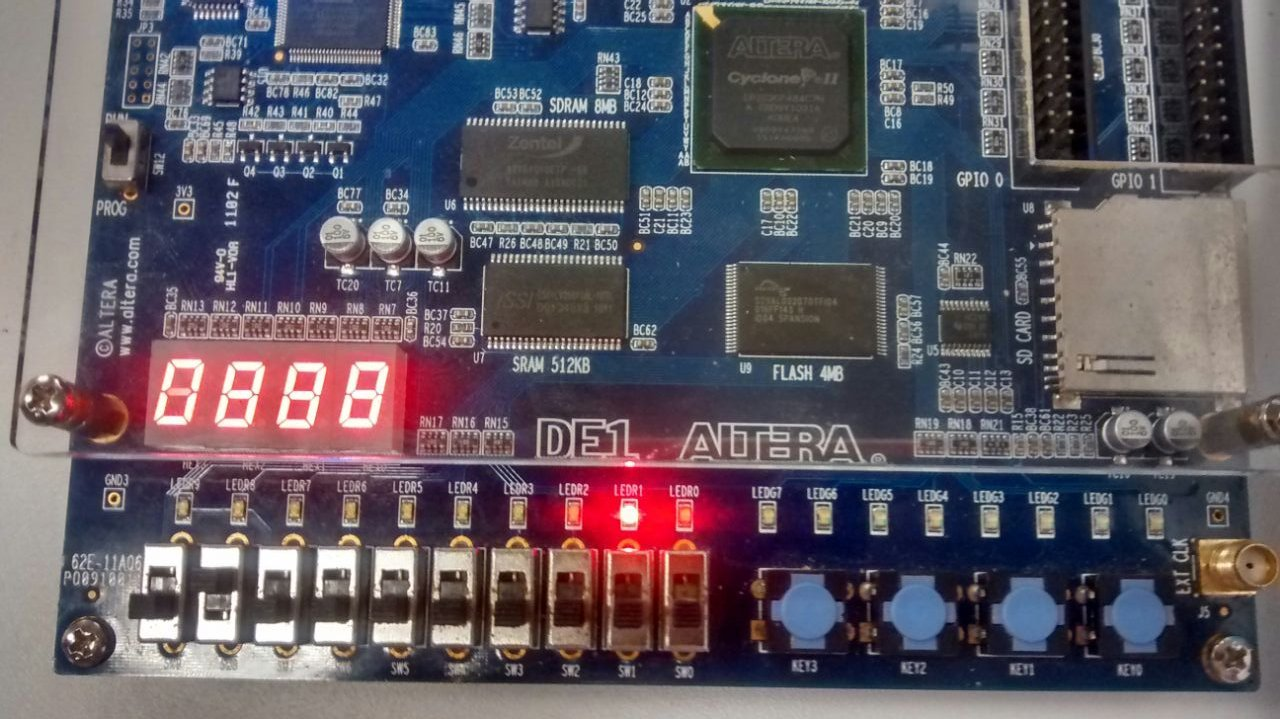
\includegraphics[width=\textwidth]{img/cenario2/circ8}
	        \label{fig:circ8}
			\caption{1 1 1 -> 1}
	    \end{subfigure}


	    \caption{Imagens do circuito na placa}\label{fig:fotosCircuito}
	\end{figure}

%Apresentar os resultados da simulação em software e da utilização do Kit DE1 e/ou
%protoboard. Utilizar figuras, descrevê-las e discuti-las.
